\documentclass{article}
\title{CSCI 447 Project 2 Design Document}
\author{George Engel, Troy Oster, Dana Parker, Henry Soule}

\usepackage{hanging}
\usepackage{graphicx}

\begin{document}
\maketitle
<<<<<<< Updated upstream

\section{Introduction} %Possible TODO: add in description of loss functions we are using to define 'accuracy'.
For this assignment, we are required to assess the performance of five different algorithms on six different data sets. The five algorithms used are $k$-nearest neighbors, edited $k$-nearest neighbors, condensed $k$-nearest neighbors, $k$-means clustering, and $k$-medoids clustering.  The essential purpose of the latter four algorithms is to produce a reduced data set with which to run k-nearest neighbors. We have found literature suggesting improved accuracy among nearest neighbor algorithms that employ data reduction [1][2].  Based on this, we have hypothesized that the average accuracy of $k$-nearest neighbors across all six data sets without reduction will be worse than the average accuracy across the six data sets once reduction has been performed via edited k-nearest neighbors, condensed k-nearest neighbors, k-means clustering, and k-medoids clustering.

\section{Class Descriptions}

\begin{center}
    \makebox[\textwidth]{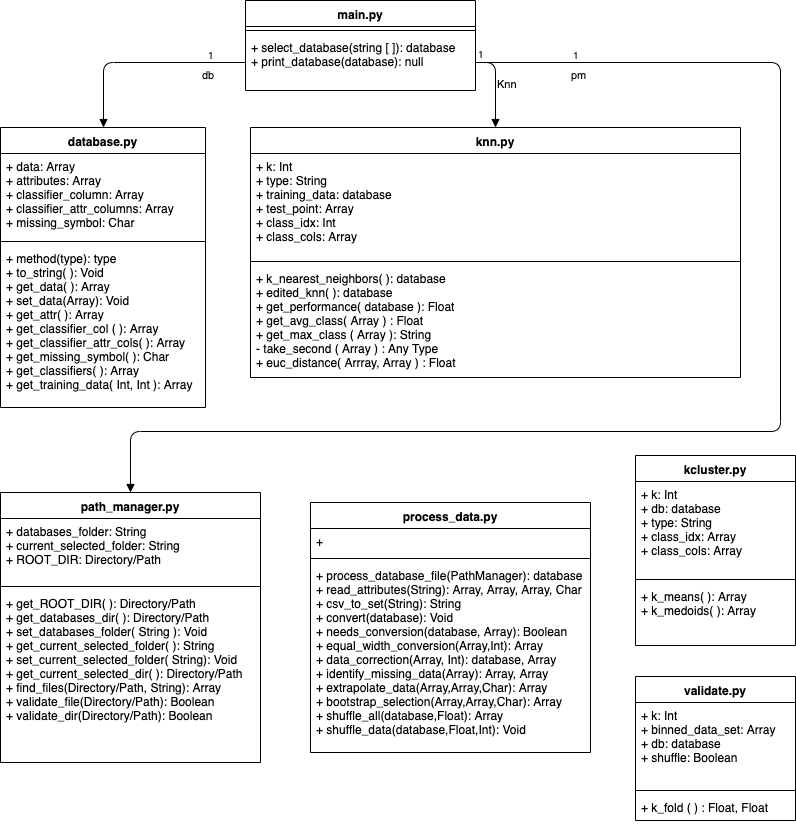
\includegraphics[width=4.75in]{uml}}
    \caption{\label{test} Figure 1: UML diagram of the files described below.}
\end{center}

\subsection*{path\_manager.py}
\texttt{path\_manager.py} handles pathing through the project's databases. This way it is easy to reconfigure or setup for a new database or file type at a moment's notice.

\subsection*{database.py}
\texttt{database.py} acts as an instantiable object for holding relevant information from a selected database (project data files).

\subsection*{process\_data.py}
\texttt{process\_data.py} makes use of the \texttt{path\_manager.py} to target a specified database, then loads in the relevant information from that database, then loads in the relevant information from that database's directory into a database object which can then be manipulated as we please. This class also contains functionality for identifying and correcting missing values from a database via bootstrapping. It also contains functionality for randomly shuffling the data of a given database by specific attribute and percentage to modify.

\subsection*{knn.py and kcluster.py}
\texttt{knn.py} will store our implementations of $k$-nearest neighbors, edited $k$-nearest neighbors, and condensed $k$-nearest neighbors. \texttt{kcluster.py} will store the implementation of $k$-means clustering and $k$-medoids clustering.

\subsection*{validation.py}
\texttt{validation.py} will perform our 10-fold cross-validation and our loss functions.

\subsection*{main.py}
\texttt{main.py} will perform the execution of our program. 

\section{Design Decisions}

\subsection*{Missing Data Handling}
When a data set is identified to have missing data, we identify the sets of data with missing attributes, and move them from the database's stored data matrix into a separate list of the sets of data with missing attributes. Once the missing data has been identified, we substitute values for the missing attribute via bootstrapping random values from the set of data that does not contain any missing attributes as our means of imputation.

We opted to never remove data, even if under a certain threshold, as we assumed it would be more likely to impact our results than including data that would be discredited if incorrect by other present data. 
Additionally, we don't have a static value to symbolize a missing value, but rather one must be specified for a given data set in the database directory's \texttt{.attr} file. This approach allows missing values to be considered a category of their own if necessary.

\subsection*{Identifying Categorical versus Continuous Data}
In order to determine how we should process data, we have decided to use our method from Project 1 for identifying categorical versus continuous data types to automatically handle which algorithms will be available to use on a given data set.

\subsection*{Nearest Neighbors Distance Function}
We decided on Euclidean distance as our means of determining nearest neighbors, as Manhattan distance didn't seem to make much sense seeing as it isn't direct. 

\section{Experimental Design}

In order to test our implementations of the algorithms, we will use classification and regression data sets as indicated in Figure 2 below. 

\begin{center}
    \makebox[\textwidth]{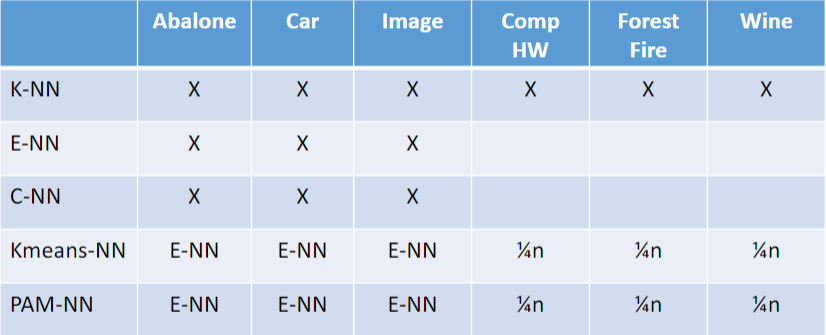
\includegraphics[width=4.75in]{chart.PNG}}
    \caption{Figure 2: Project 2 Clarification chart}
\end{center}

For each test, we will use 10-fold cross validation with the equal width binning approach for setting up the training and testing bins from the given data set.

\subsection*{Handling Tuning}

We will be following the rule of thumb to use the square root of the number of training samples as the initial value for the amount of neighbors, $k$, used for the nearest neighbors algorithms.[3] From here we want to see if we can improve our ability to more accurately represent the model by increasing and decreasing the value of $k$ and checking if it is a better fit.

However, it is worth noting that this method is susceptible to the hill climbing problem. Unfortunately, working our way around that with more iterations would likely result in a drastic increase in the amount of time it takes to find the supposed "optimal" $k$ value, so we may not end up with a perfect solution as we will likely forgo this additional step.

\subsection*{Evaluation}

In order to properly evaluate our implementations, we will split up our evaluation methods for regression- and classification-based problems into separate functions. This is necessary seeing as classification-based methods don't involve continuous values, whereas the regression-based methods do, hence the innate disconnect and reasoning for identifying and evaluating them separately.

For evaluating our regression-based algorithms, we need a way of comparing our method's predicted continuous value to the actual continuous value. But we also need a method of measuring our prediction accuracy that is robust to outliers. So, we decided to use Mean Absolute Error (MAE), which measures the sum of the absolute differences between our predicted continuous values and the actual continuous values, and then averages the result by the number of values compared. ($MAE = \frac{1}{n} \sum_{i=1}^n | y_i - \hat{y}_i|$). It is important that MAE averages the absolute difference, because then MAE will be resistant to outliers because it weighs the individual differences equally.[3] The closer MAE is to 0, the better our predicted line of best fit.

As for evaluating how well our classification algorithms perform, we need a way of comparing our predicted classifications against the actual classifications. So, we decided use the Mean Squared Error (MSE) as it tells us how far off our prediction distribution is from the actual distribution and the accuracy as metrics for algorithm evaluation. The smaller the result of MSE is, the better our ability to accurately predict the correct classification.  We use accuracy in addition because MSE on its own can possibly be 0 on its own which would lead to incorrect classifications.

=======
\section{Introduction}
For this assignment, we are required to assess the performance of five different algorithms on six different data sets. The five algorithms used are $k$-nearest neighbors, edited $k$-nearest neighbors, condensed $k$-nearest neighbors, $k$-means clustering, and $k$-medoids clustering.  The essential purpose of the latter four algorithms is to produce a reduced data set with which to run k-nearest neighbors. We have found literature suggesting improved accuracy among nearest neighbor algorithms that employ data reduction [1][2].  Based on this, we have hypothesized that the average accuracy of $k$-nearest neighbors across all six data sets without reduction will be worse than the average accuracy across the six data sets once reduction has been performed via edited k-nearest neighbors, condensed k-nearest neighbors, k-means clustering, and k-medoids clustering.
%Possible TODO: add in description of loss functions we are using to define 'accuracy'.
\section{Experimental Design}
%UML DIAGRAM GOES HERE%
\subsection*{Components}
Our design has 5 primary components. $database.py$ is a wrapper class that will handle all functionality of each data set. Each instance of the database class will store the processed data of one our six data sets, the the index of the class attribute of its respective database. $knn.py$ will store our implementations of $k$-nearest neighbors, edited $k$-nearest neighbors, and condensed $k$-nearest neighbors. $kcluster.py$ will store the implementation of both clustering algorithms--$k$-means and $k$-medoids clustering. $validation.py$ will perform our 10-fold cross validation and our loss functions. $main.py$ will perform the execution of our program. 
\subsection*{Design Decisions}
Each of the five algorithms we are implementing compute distance between data points in each data set. We have chosen to use Euclidean distance for each algorithm. We will be using 0-1 Loss to compute performance of each algorithm on each classification data set. We will use Mean Squared Error to compute performance of each algorithm on each regression data set. %TODO K values%
\section{Plan}
To test our hypothesis, we need to compute the average performance of $k$-nearest neighbors across all six of our data sets, and the average performance of each of the other four algorithms across all six data sets. Our program will first perform $k$-nearest neighbors on all six our data sets, performing 10-fold cross validation for each data set. As we perform our cross-validation for $k$-nearest neighbors on each data set, we will compute the average loss function (0-1 Loss for classification data, Mean Squared Error for regression) for the current data set. We will then compute the average overall loss function across all six data sets once we have completed our cross validation for each data set. \\ \\
We will then perform 10-fold cross validation using the four other algorithms. Each of these algorithms produces a reduced data set with which to work. Thus, we will implement each of these algorithms to output the reduced data set. For each of the reduced data sets produced by each of the four algorithms, we will perform 10-fold cross validation.
>>>>>>> Stashed changes

\section{Works Cited}
\begin{hangparas}{.25in}{1}
[1] Wagner, T. "Convergence of the Edited Nearest Neighbor (Corresp.)." IEEE Transactions on Information Theory, vol. 19, no. 5, 1973, pp. 696?697., doi:10.1109/tit.1973.1055059.

[2] Nitin Bhatia, V. "Survey of Nearest Neighbor Techniques.: International Journal of Computer Science and Information Security, vol. 8, no. 2. 2010.

[3] Drakos, Georgios. “How to Select the Right Evaluation Metric for Machine Learning Models: Part 1 Regression Metrics.” Medium, Towards Data Science, 5 Dec. 2018, https://towardsdatascience.com/how-to-select-the-right-evaluation-metric-for-machine-learning-models-part-1-regrression-metrics-3606e25beae0.
\end{hangparas}

\end{document}